% Edit the title below to update the display in My Documents
\title{Project Report}
%
%%% Preamble
\documentclass[12pt,a4paper]{article}
\usepackage[legalpaper,bottom=4cm]{geometry}
\usepackage[T1]{fontenc}
\usepackage{lmodern}
\usepackage[english]{babel}	% English language/hyphenation
\usepackage[protrusion=true,expansion=true]{microtype}	
\usepackage{amsmath,amsfonts,amsthm} % Math packages
\usepackage[pdftex]{graphicx}
\usepackage{subcaption}	
\usepackage{url}

%% Bibliography
\usepackage[natbib=true,backend=biber,bibencoding=utf8,doi=false,isbn=false,url=false]{biblatex}
\usepackage{csquotes}
\addbibresource{references.bib}
\AtBeginBibliography{\small}

\renewcommand{\baselinestretch}{1.2}

%%% Custom sectioning
\usepackage{sectsty}
\allsectionsfont{\normalfont\scshape}


%%% Custom headers/footers (fancyhdr package)
\usepackage{fancyhdr}
\pagestyle{fancyplain}
\fancyhead{}			% No page header
\fancyfoot[L]{}			% Empty 
\fancyfoot[C]{}			% Empty
\fancyfoot[R]{\thepage}	% Pagenumbering
\renewcommand{\headrulewidth}{0pt}	% Remove header underlines
\renewcommand{\footrulewidth}{0pt}	% Remove footer underlines
\setlength{\headheight}{13.6pt}


%%% Equation and float numbering
\numberwithin{equation}{section}	% Equationnumbering: section.eq#
\numberwithin{figure}{section}		% Figurenumbering: section.fig#
\numberwithin{table}{section}		% Tablenumbering: section.tab#


%%% Maketitle metadata
\newcommand{\horrule}[1]{\rule{\linewidth}{#1}} 	% Horizontal rule

\title{
		%\vspace{-1in} 	
		\usefont{OT1}{bch}{b}{n}
		\normalfont \normalsize \textsc{Building and mining knowledge graphs} \\ [25pt]
		\horrule{0.5pt} \\[0.4cm]
		\huge Creating and completing a graph about music \\
		\horrule{2pt} \\[0.5cm]
}
\author{
		\normalfont 								\normalsize
        Adrian Rodriguez Grillo - 6193748\\[-3pt]		\normalsize
        \today
}
\date{}

%%% Begin document
\begin{document}
\maketitle

\section{Introduction}
With regards to the distribution of the music, internet has become the platform that provides the greatest revenues, being 2017 the first year that it accounted over the half of the total revenues generated \citep{music_report_2018}.
This platform presents a great opportunity to all kind of artist but, at the contrary of what happened in the past, the entry barrier is much lower.
Nowadays, amateur and alternative artists can upload their music to the cloud to make themselves known without having to depend from a record and start their musical career. 

However, in order to be discovered by a broader audience, the information about these artists has to be complete and correct.
Only in that way, a better position in the search engines and in the recommendations will be achieved.
Although some of this data depends of closed services where the music can be uploaded, there also exist public domain knowledge platforms like Wikipedia \citep{wikipedia}, Wikidata \citep{wikidata}, DBpedia \citep{dbpedia} or, more specialized ones, like MusicBrainz \citep{musicbrainz} that facilitates the publication of this information and which are used to generate results for the users. 

In any case, including a complete and consistent information across the different platforms requires a dedication that most of this kind of artists cannot afford, leading to situations where the data differs between websites or, directly, is missing.
In this project, the consistency of the information among different public domain platforms and the completion between each other were assessed using knowledge graphs.
Firstly, creating a knowledge graph from the MusicBrainz music database that, later, was linked and completed with others open data KGs, Wikidata and DBpedia. 
\section{Definition of Knowledge Graph}
When it comes to define what is a Knowledge Graph (KG), both in the academic and business world, there is not a consensus about the characteristics required to fulfil the definition.
As it is explained in \citet{Ehrlinger2016} a great variety of definitions have arisen in the last years with the developments made in this field.
In this project, a knowledge graph will be created from a relational database and will be compared and completed with the information contained in other known open knowledge graphs. 

We are going to define a knowledge graph as an information storage system where the content is described and interrelated forming a network that can be seen as a graph.
Following the mathematical definition of graph, in a knowledge graph there will be vertices, which in a KG will represent the entities, and edges, which will represent the relation between entities.  

An entity is the representation of an independent thing, like a person, a place or an object, that will belong to a type defined by an ontology and will have some properties that will describe it.
An example could be the entity ``Dave Grohl'', whose type will be ``musician'' that will be defined by an ontology and will have some properties like the name and surname that will describe the entity. 

On the other hand, an edge will represent the relationships between different entities contained in the knowledge graph.
These relationships will be also defined by an ontology and are the only way of directly relate two independent entities.
Continuing with the previous example, ``Dave Grohl'' will be associated with the entity ``Foo Fighters'' with the relation ``is member of'', that in this case, also generates the inverse relation ``Foo Fighters'' has ``Dave Grohl'' as a member of the group. 

The use of the relationships will also allow the connection of the information contained within the knowledge graph with other external sources, in a process known as interlinking.
Moreover, apart from representing information, a KG will allow the extraction of new knowledge through the exploitation of the relationship between entities and external sources. 

In this project, the Resource Description Framework (RDF) will be used to generate the graph.
The main difference of this kind of graph regarding property graphs is that the relationships between entities do not contain properties.  
\section{Problem}
A great quantity of information about artists and music exist on the internet, however, depending on the platform visited or the search provider used the data could vary, making the information inconsistent and incorrect.

In general, most of this information comes from private companies that are dedicated to the music business, like Spotify \citep{spotify} or Last.fm \citep{lastfm}, that provide more accurate and correct data but that is not always the case. Moreover, the data is not freely available and is usually being subjected to some conditions, so the correction of it is not an easy or possible task.  

On the contrary, search engines and music platforms also work with the information contained in open data portals, like Wikipedia or MusicBrainz, where a great quantity of the information is crowdsourced and, in the case of music, generated by fans.  

Even though these pages have control mechanisms to verify the data uploaded, is easy to find the problems described previously. For example, there are situations where the genres of a band differ between sites or where some information is missing in some but not others at it can be appreciated in the figure \ref{fig:data-comp}.

\begin{figure}[t!]
	\centering
	\begin{subfigure}{0.46\columnwidth}
		\centering
		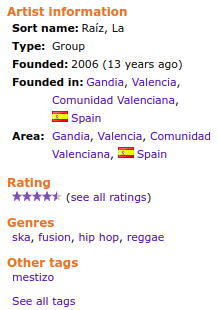
\includegraphics[width=0.7\linewidth]{images/mb-laraiz.png}
		\caption{La Raiz information in MusicBrainz.}
		\label{subfig:raiz_mb}
	\end{subfigure}
	\begin{subfigure}{0.46\columnwidth}
		\centering
		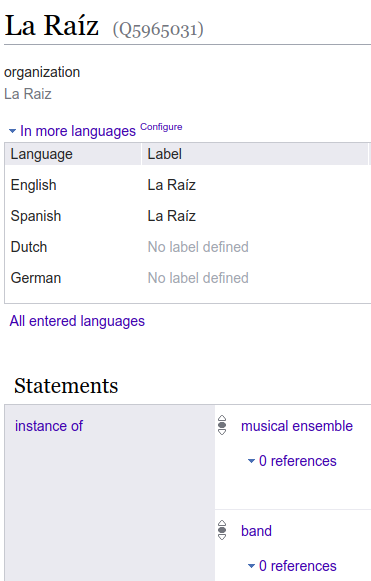
\includegraphics[width=0.63\linewidth]{images/wd-laraiz.png}
		\caption{La Raiz information in MusicBrainz.}
		\label{subfig:raiz_wd}
	\end{subfigure}

	\caption{Comparison between the data of (\textbf{a}) MusicBrainz and (\textbf{b}) Wikidata.}
	\label{fig:data-comp}
\end{figure}
\section{Significance}
As a passionate fan of alternative music and, specially, of small groups of my country, it can be seen how these inconsistencies usually occurs among the different platforms, leading to incorrect results or non-related recommendations.
Problems like these can generate frustration between the users, reducing the chances of the artists to being discovered. 

Generally, most of the inconsistencies are found in alternative artists that do not have the resources to fix this situation by themselves, therefore, any help this kind of groups can receive is extremely valuable for them as it increases the probability of reaching a broader audience.

Moreover, as a defender of open data and crowdsourced information, I believe that any project that can help or give ideas on how to improve the quality of the data are extremely important nowadays.
Especially if it is focused in the consolidation of the data in order to make the information reliable and improve the perception of this platforms as a trustworthy source.
\section{Methodology}
In order to solve the issue previously mentioned through the use of knowledge graphs, the differences of the information contained among different open data platforms will be assessed and a way to complete the information between sources will be studied and tried.  

Three different sources will be used in this project. MusicBrainz, the music database, will be the main source of the information whereas DBpedia and Wikidata will be used to analyse the differences and complete the information of the original information.  

Therefore, the project will be divided in two different phases: firstly, the knowledge graph will be generated from the database information and, secondly, different ways to interlink and complete the data will be analysed and used in order improve the original information. 
\section{Related work}
Different projects had used the MusicBrainz dataset to generate a knowledge graph in order to improve the connectivity with the linked data initiative, however they have been discontinued because of the lack of resources.
Nevertheless, some official information exists about the process of generating a graph \citep{musicbrainz_map} and, also, a non-official SPARQL endpoint \citep{musicbrainz_endpoint} 

Especially remarkable is the \citet{musicbrainz_map} project, that provides the mapping files and some scripts to generate the KG directly. This work was considered to quickly generate the graph for this project and focus in the linking and completion task. However, due to the unavailability of the tool required in the execution and the outdated structure of the mapping files, the generation of a new knowledge graph was undertaken. 

Linking knowledge graphs have been a widely covered topic and one of the main purposes of the semantic web. Tools like LIMES \citep{limes} and the Silk \citep{silk} framework facilitates the task of interlinking different knowledge graphs and in \citet{linking_book} a review all the principles related with the task can be found. Additionally, there have been some efforts to use external and unstructured information to expand and improve existent knowledge graphs. 

Although in \citet{refinement_survey} the possibility of using interlinked data is contemplated to complete the knowledge graph information, the mentioned approaches effort goes into predict either missing entities, missing types for entities, and/or missing relations that hold between entities. However, there is not much work that covers the problem of completing and filling the information of existent entities with the use of external sources.
\section{Development}
In this section, the steps and actions taken to develop this project will be briefly described\footnote{A detailed explanation of the development can be seen at \url{https://github.com/adrigrillo/music_kg/issues?q=is\%3Aissue+is\%3Aclosed}}.
As it was outlined in the methodology method, the work can be divided in two parts, the creation and the interlinking and completion of the graph.

\subsection{Graph creation}
The selection of the MusicBrainz database to generate the knowledge graph was due to its specialization in music, that was the topic of interest for this project.
Unlike DBpedia or Wikidata, that are general graphs, MusicBrainz focuses only in the music having a rather complex but clear schema\footnote{\url{https://beta.musicbrainz.org/doc/MusicBrainz_Database/Schema}}, where all the entities and properties are clearly defined.
To create the knowledge graph from the MusicBrainz data various prerequisites were required.

First, it was necessary to have all the information at hand.
This was achieved using the virtual image provided by the platform, that generates a slave node of the database with replication capabilities.
Event tough this option required a lot of time to reach the update state of the database, it was selected because other options either make to configure a full database, to import a dump, or was a rate limited endpoint.

Secondly, a scalable tool to generate the triples (.nt) from the database information was required.
Because of the limitation of the RMLMapper \citep{rmlmapper} project that saves intermediate results in memory, the project R2RML was picked to generate the output from the mapping files. 

Lastly, the mapping files had to be created to make the tool work.
Due to the time limitations of the project and the complexity of analysing all the database schema, only mapping files for the artists, genres and areas where generated.
Except for the genres, a mapping file is composed by a set a SQL queries that extract some information and a set of statements that generate the graph entities, with an identifying URI and a set of properties.

Different ontologies and vocabularies where used in the creation of the graph in order to follow a standardized way.
Due to the music specialization of the project, The Music Ontology \citep{music_ontology} is the default model of the graph and is used to define the artist and the genres.
However, it has its limitations to define other non-related entities, like the areas, and, so, other ontologies like the LinkedGeoData \citep{linkedgeodata} where used. 

Different decisions were taken during the creation of the mapping files depending of the entity to map:

\subsubsection{Areas (\textit{area-mapping.ttl})}
The areas table in MusicBrainz describes the zone where the artists come from and, also, to situate places, like recording studios, festivals, etc.
They are divided using a hierarchical relation were the countries are the root for all the relations, this is, any area is connected directly or indirectly to the countries.  

Due to the richness in concepts of the LinkedGeoData ontology, it was possible to designate a type of entity to each of the different types of area of the database.
Moreover, the relation between entities was modelled in a smaller to bigger category way, using the is part of definition.
In general, an area instance is composed by an URI, used as id, the type of area is it, the official name and a list of aliases that are used. 

\subsubsection{Genres (\textit{genres-mapping.ttl})}
The genres in the MusicBrainz database are hardcoded in the server, in a way that an artist has a set of tags where, apart from the genres, user created elements coexist.
However, a list with the genres accepted in the database is available and was used to generate this part of the graph.
Because there is not a page that describe the genres, the URI generated for these instances is invented. 

\subsubsection{Artist (\textit{artist-mapping.ttl})}
The artists part was the most complex to model because of the high number of relations that can be found. In this case, MusicBrainz generates a distinction between individuals and groups that will be used to classify the entities between the definitions of \textit{MusicArtist} or \textit{MusicGroup}. Depending of the kind of entity the properties of those changes, musicians have a gender and the dates indicates the birth and death year whereas groups do not have gender and the dates highlight the foundation and dissolution years. 

Because the MusicBrainz database is specialized in music, not only the information of the groups is available but also the information about their components, that are instances also. This situation was handled with the definitions of \textit{member} and \textit{supporting\_musician}. Additionally, to add more information to the graph, the collaborations between artist were also added. 

\subsubsection{Artist-Genre relation}
As it was mentioned before, the artists are linked to a set of tags where the genres are included along other user-generated words.
To solve this situation and generate a relation between the artist and the genre entities the following process was followed:

\begin{enumerate}
\item All the tags of the artist were included as a property using the tag string. This is provided in the file \textit{artist-mapping\_with-tag.ttl} in the triples map called \textit{\#GenresTriples}.

\item A SPARQL query (\textit{1\_artist-genre-relation.txt}) was used to generate the triples that link the artist and the genre matching the name of the tag with the name of the genre.

\item All the tags from the artist were removed of its properties as they do not provide valuable information.
Additionally, a SPARQL query (\textit{2\_empty-artists-remove.txt}) were ran to remove invalid artist-genre relations.
\end{enumerate}

This method was required because of the incompatibility of generating a URI with the R2RML tool as strange characters were included in the tags string, like Chinese words and Unicode emojis. 
The file \textit{artist-mapping.ttl} contains all the artists triples without including the tags.

Regarding the general process of creation of the knowledge graph, an overview of the composition of the graph and the content will be further developed in the next section.

\subsection{Interlinking and completion}
Although interlinking and the completion of the data are two different tasks, in this case, they are tightly related as the same kind of situation were found during the execution of the tasks.
The external sources used to improve the quality of our previously generated graph are Wikidata and DBpedia, that are general purpose open access knowledge graphs maintained by their respective communities and that allow any user to add information. 

In this part of the project, the genres are the part of the graph where most of the attention were put because of the lack of content and context available in the original information.

\subsubsection{Interlinking}
The interlinking task was done using LIMES, that allows the linking of two different knowledge graphs with the use of SPARQL. The configuration files for the linking process between genres of the original graph and the ones of Wikidata and DBPedia can be found in the files \textit{genres\_wikidata-config.xml} and \textit{genres\_dbpedia-config.xml} respectively.  

The interlink between artist was also tried without successful results, a configuration to relate the groups of the graph with DBpedia can be found in the file \textit{groups\_dbpedia-config.xml}. Further discussion about this results will be developed in the following section.

\subsubsection{Completion of the graph}
The completion of the existing graph where performed with the use of different double-sided SPARQL queries, that perform their work in more than one graph. 
In this case the connected graphs were the original MusicBrainz graph and Wikidata or DBpedia.
As in the previous case, this work focused in the genres part of the graph, setting two different objectives. 

Firstly, after an examination of the genres present in the external sources, whose number was superior, the decision of including the missing genres in the original graph was taken.
This process implied the query and comparison of all the genres contained in the external sources in order to include the ones missing.  

Due to the clear definitions of the genres in both of external sources, this process was simple and limited to the extraction of all the entities of the type \textit{genre} and its names.
Additionally, due to the previous linking process the discarding of the already present genres was made comparing the URIs, if existent. Otherwise, a matching in the was used.
The queries of this process can be found in the files \textit{2\_wd\_add-new-genres.txt} and \textit{3\_db\_add-new-genres.txt}. 

Secondly, as having instances in a graph with any kind of relation does not generates any value, the following step was to relate the existent artist with the new genres. The only way to accomplish this task was through the use of the external graphs, that were the source of the information. 

Using SPARQL, the approach followed extracts all the artists linked to the genre of interest and generates a relation between them if and only if both exist in the graph. Regarding the matching of the artist of the original knowledge graph and the external source, two different approximations were tried: 

\begin{itemize}
\item Using only the name of the artist to generate the relation. This approach can be found in the files \textit{5\_db\_relate-artist-genres.txt} and \textit{6\_wd\_relate-artist-genres.txt}

\item A stricter approach, that uses a specific property of the artist to make the relation between the two sources. It can be found, using the year of foundation, in the file \textit{7\_db\_relate-artist-genres-year.txt}.
\end{itemize}

The results of this process will be developed further in the next section.
\section{Findings and results}
As an overview of the overall project, the resulting knowledge graph\footnote{The output files of the graph can be found in: \url{https://1drv.ms/f/s!AnzM-42un3oRrHHXYaTQIesWyNtB}} generated contains more than seven million of statements.
To imagine how big this graph could have become, it is worth remembering that only the information related with the artists, genres and locations from the original dataset was used to generate the graph.
Moreover, with respect of the MusicBrainz database, there exist more than twenty million of albums and tracks instances.

\begin{figure}[!tbh]
\centering
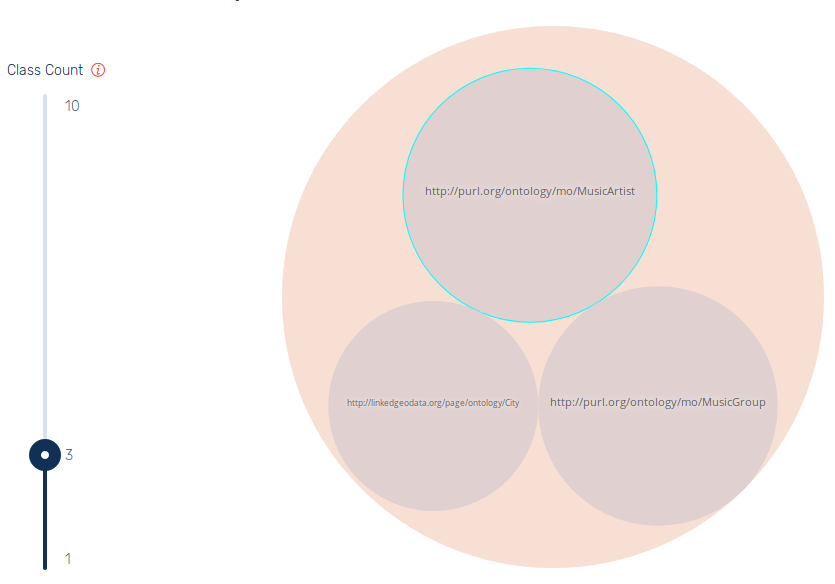
\includegraphics[width=0.8\linewidth]{images/classes}
\caption{Entity types with the greatest number of instances of the graph.}
\label{fig:classes}
\end{figure} 

Regarding the composition of the graph, entities of ten different classes exist, being \textit{MusicArtist}, \textit{MusicGroup} and \textit{City} the three with more instances (figure \ref{fig:classes}). In the subfigure \ref{subfig:green_day}, a graphical example of the knowledge graph can be appreciated showing the information of a rather complete music group. The example shows most of the possible relations that can be found, having as the centre node a group band, it is related with some genres (yellow), their members and supporting musicians (purple) and the area it comes from (blue).

\begin{figure}[!tbh]
	\centering
	\begin{subfigure}{\columnwidth}
		\centering
		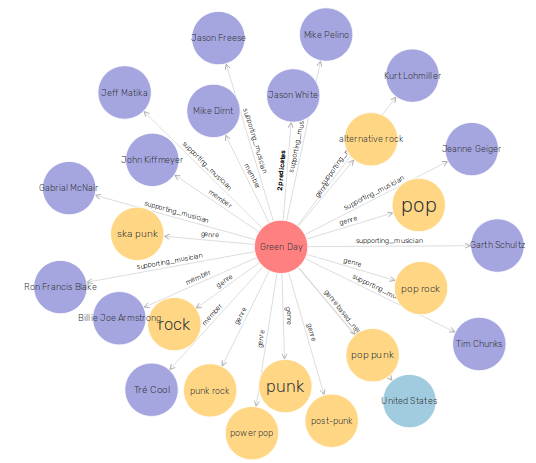
\includegraphics[width=0.8\linewidth]{images/greenday.png}
		\caption{Green Day information in the knowledge graph.}
		\label{subfig:green_day}
	\end{subfigure}
	\begin{subfigure}{\columnwidth}
		\centering
		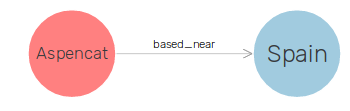
\includegraphics[width=0.5\linewidth]{images/aspencat.png}
		\caption{Aspencat information in the knowledge graph.}
		\label{subfig:aspencat}
	\end{subfigure}

	\caption{Comparison between (\textbf{a}) known and commercial artist and (\textbf{b}) alternative artist.}
	\label{fig:graph-comp}
\end{figure}

After the analysis of the knowledge graph, one of the findings that confirms the belief of the alternative groups having less complete information in these open platforms can be appreciated in figure \ref{fig:graph-comp}.
It is clear that, comparing the information presented in the subfigure \ref{subfig:green_day} with respect the subfigure \ref{subfig:aspencat}, the first is much more complete whereas in the second only the origin area is shown. 

Other aspect worth discussing in this section are the results obtained in the interlinking and completion tasks.
During the development of this phase, two opposed situations were found.
On the one hand, the work made with respect to the musical genres was successful and returned great results.
For example, from the original 419 genres contained in MusicBrainz, 368 were linked with Wikidata and 291 with DBpedia, meaning a success superior to the 70\% in both cases.

The previous situation was repeated for the completion of the genres, were 1217 of the 1568 original Wikidata genres were added and 389 of the 1245 of the DBpedia ones. 
These cases were favoured due to the use of a clear and stable set of definitions for the entities. 

On the other hand, the interlinking and completion tasks that were related to the artists and the areas did not turn that well.
Two reasons lead to these results, the entity definitions used in both sources to refer to music artists and the existence of different entities with the same name.  

Regarding the first situation, in the case of Wikidata, a music artist can have a wide range of types as its class definition due to the use of genres in them. 
For example, a music group like ``Green Day'' is defined like a \textit{rock band} whereas another similar band like ``blink-182'' is defined only like a \textit{band}.
This difficult greatly the possibility of generating a generalized way to complete the data among graphs, as the queries became very specific. 

The second situation\footnote{More details can be found in: \url{https://github.com/adrigrillo/music_kg/issues/8\#issuecomment-477783435}} is impossible to avoid due to the fact that a name cannot be considered a unique id for the different entities.
This kind of case can be solved with the use of more information related to the artist, like the year of foundation (\textit{7\_db\_relate-artist-genres-year.txt}).
However, this can be problematic when some of the data is missing in one of the datasets, or directly, in both, as there is no way to validate the relation.

\begin{figure}[!tbh]
	\centering
	\begin{subfigure}{\columnwidth}
		\centering
		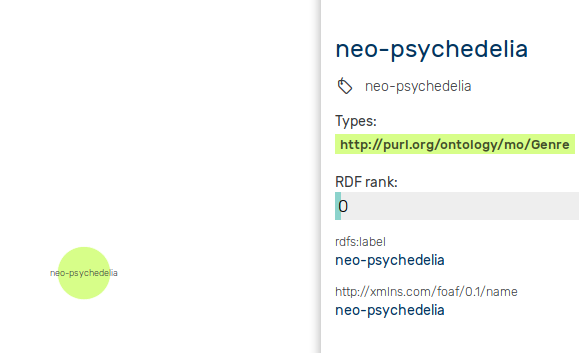
\includegraphics[width=0.7\linewidth]{images/neo-psychedelia.png}
		\caption{Before the completion task.}
		\label{subfig:before}
	\end{subfigure}
	\begin{subfigure}{\columnwidth}
		\centering
		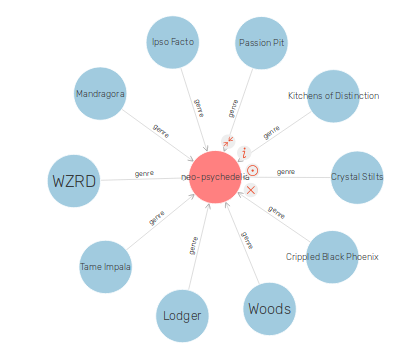
\includegraphics[width=0.63\linewidth]{images/neo-after.png}
		\caption{After the completion task.}
		\label{subfig:after}
	\end{subfigure}
	\caption{Information of a genre (\textbf{a}) before and (\textbf{b}) after the completion task that relates artist with the new genres.}
	\label{fig:completion}
\end{figure}

As an example, the query that used the year of foundation correctly linked 1385 artist with the new genres, completing the graph as can be seen in figure \ref{fig:completion}, but the number is low compared with the million of artist present in the graph. 

Consequently, both of the described situations lead to the specialization of the queries in order to achieve correct results and moves them away of the objective of finding a generalized way to complete knowledge graphs. Moreover, this finding could be one of the reason because there is not much development in this topic. 
\section{title}
\section{Conclusion}
In this project, two related but differentiated task were carried out and described, the creation of a knowledge graph from a relational database and the linking and completion of a knowledge graph with the use of other external graphs. 

Regarding the first task, it can be concluded that the difficulty of generating a graph from a relational database will depend greatly on the scheme complexity. 
As the mapping tool requires a tabular input, such a table or the selected attributes of a query, obtaining the information necessary to generate a relation between two different type of entities could implicate the creation of complex queries.  

Nonetheless, other aspect to remark is the superiority of the knowledge graph to represent some relations between entities with respect to the relational databases.
A clear example could be the ``member'' relation that exist between music groups and musicians, that is direct in the knowledge graph generated whereas to extract this information in the database the join of three different tables is required \footnote{\href{https://github.com/adrigrillo/music_kg/blob/master/queries/sql/query-artist.sql}{SQL queries} used to generate the mapping of the artists}.  

With respect the interlinking and, specially, the completion of the graph with external sources, this project highlights the difficulty of finding a generalized way to relate entities of different datasets. 
This complexity not only comes from the lack of common vocabularies and structures among knowledge graphs but also from the inherent nature of the things, with a clear example in the existence of two different kind of entities with the same name. 

%%% Bibliography
{\tiny\printbibliography}
%%% End document
\end{document}